

\documentclass{pracalicmgr2021}
\usepackage{chngcntr}
%\counterwithout{figure}{chapter}
\counterwithout{table}{chapter}
\counterwithout{equation}{chapter}
\usepackage{polski}
\usepackage[utf8]{inputenc}
\usepackage{indentfirst}
\usepackage{graphicx} 
\bibliographystyle{unsrt}
\usepackage{notoccite}

\author{Mikołaj Boroński}

\nralbumu{418365}

\title{Classification of signals from gravitational waves detectors using spiking neural networks}

\tytulang{Classification of signals from gravitational waves detectors using spiking neural networks}

\kierunek{Zastosowania Fizyki w Biologii i Medycynie}

\specjalnosc{Neuroinformatyka}

\opiekun{dr hab. inż. Piotr Gawron \\ AstroCeNT, Centrum Astronomiczne im. Mikołaja Kopernika PAN}

%\dziedzina{13.200}
%\dziedzina{13.2 Fizyka}

\date{czerwiec 2022}

\keywords{fale grawitacyjne, klasyfikacja, sieci pulsujące}

\begin{document}


    \maketitle
    \let\cleardoublepage\clearpage
    
    \begin{abstract}
    Streszczenie pracy licencjackiej
    \end{abstract}

    \tableofcontents

    \chapter{Introduction and motivation}
    \section{State of deep learning}
    Ever since the introduction of the idea of deep learning methods in 1960s, the scientific community has been striving for better and more efficient artificial networks architectures. Using classic artificial neural networks we reached the point at which trained models can not only learn basic machine learning tasks like classification and segmentation, but also out compete people in games way more complicated then chess -- Dota, StarCraft 2, Go, write poetry and songs, create images out of text and more. 
    
    Above wouldn't be possible without increasing the number of learnable parameters. The StarCraft 2 playing model AlphaStar has 139-milion learnable parameters, image generating model DALL·E 2 tops it with 3.5-billion, but all are being dwarved by language processing models like GPT--3 at 176-billion and Megatron-Turing NLG 530B at 530-billion\cite{alphastar, dalle, gpt, megatron}. This way we can clearly see that more complicated tasks call for a higher number of parameters. Training those models wouldn't be a problem, if not for the earth's limited resources. It takes around 190,000 kWh to train GPT--3 alone\cite{energy}. 
    
    \section{The problem of energy efficiency in von Neumann architecture}
    
    \section{Spiking Neural Networks as a natural step forward}
    
    \section{In pursuit of consciousness}
    
    \section{Overwhelming amounts of data}
    
    
    \chapter{Theory of Spiking Neural Networks}
    \section{Overview}
    
    \section{Spiking Neurons}
    
    \section{Input encoding}
    
    \section{Output decoding}
    
    \section{Training and learning rules}
    
    
    \chapter{Gravitational waves}
    \section{Overview}
    
    \section{Detectors}
    
    
    \chapter{Analysis}
    \section{Data overview}
    
    \section{Data preparation}
    
    \section{Network architecture}
    
    \section{Results -- params1}
    
    \section{Results -- params2}
    
    \section{Results -- params3}
    
    
    \chapter{Summary}
    

%         Fale grawitacyjne to zaburzenia czasoprzestrzeni generowane przez każde przyśpieszające ciało posiadające masę. \cite{Einstein} 
        
%     Według człowieka, który na swoim najpopularniejszym zdjęciu pokazuje język, nigdy nie będziemy w stanie ich zaobserwować, a w konsekwencji nie docenimy jego geniuszu --- otóż mylił się, przynajmniej co do pierwszego. \cite{Abbot}  

  
%     \section{Zderzenie binarnych czarnych dziur}
        
%         Zmniejszanie się średnicy okręgu, po którym krążą zderzające się czarne dziury można opisać zależnością od czasu (Wzór \ref{wzór}). Należy jednak znać początkowy promień ($ r_o $) oraz czas do zderzenia ($ t_{zderzenia} $), który wedle mojego zegarka nastąpi wynosi mniej niż czas potrzebny do napisania tej pracy.
        
        
% \begin{equation}
% \label{wzór}
% r(t) = r_o (1-\frac{t}{t_{zderzenia}})^{1/4}
% \end{equation}
   
%     Przykładowe dane pochodzące z detektorów czarnych dziur (Rysunek \ref{sygnał}) uzmysławiają nam bezkres wszechświata i bezsens kryjący się w pisaniu pracy licencjackiej.
   
   
%     \begin{figure}[hb]
% \begin{center}
% \label{sygnał}
% \resizebox{8cm}{!}{
% 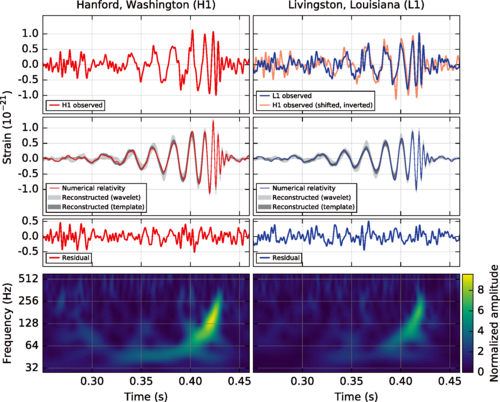
\includegraphics{medium.png}
% }
% \caption{Przykładowa analiza zarejestrowanych fal grawitacyjnych \cite{Abbot} }
% \end{center}
% \end{figure}

        
%     \chapter{Sieci Pulsujące}

% Sieci pulsujące to kolejna komiczna nazwa, która została skrzywdzona polskim tłumaczeniem. Sieci te opierają się o założenie enkodowania danych do postaci impulsów oraz ich umiejscowienie w czasie.  \cite{Ghosh}


% Wagi na połączeniach synpatycznych są liczbami zmiennoprzecinkowymi, co widać w Tabela \ref{tabela}.

% \begin{table}[h]
% \centering

% \caption{Przykładowa konfiguracja sieci}
% \begin{tabular}{||l||c||} \hline \hline
% Numer połączenia & Waga [$1$]\\
% \hline
% \hline
% 1 & 0,171\\
% \hline
% 2 & 0,271\\
% \hline
% 3 & 0,314\\
% \hline
% 4 & 0,420\\
% \hline
% \end{tabular}
% \label{tabela}
% \end{table}
%     %\chapter{Metodologia}
%   % \chapter{Wyniki}
   
%     %\chapter{Dyskusja}
%   % \chapter{Podsumowanie}

\bibliographystyle{plain}
\bibliography{bibliografia}
\end{document}

